\chapter{Tree Refinement}
\label{chap:tree}
% 0.5 Seiten

	With the existing capabilities of \ac{GCG} presented in the previous chapter, we continue with the main contributions of this thesis:
	
	\begin{itemize}
		\item A new module which is integrated into the detection framework of \ac{GCG} for reverse engineering semantic groupings of the original formulation.
		\item Additional auxiliary classifiers which implement constraint and variable classification based on information not currently used including examples of \textit{when} they are crucial detecting semantics.
	\end{itemize}

	This chapter is divided into three main section:
	
	\begin{enumerate}
		\item A short summary about the available information we have access to.
		\item What the motivation and goals are why and how we aim to process this information.
		\item The concrete algorithm and its most integral parts.
	\end{enumerate}
	
	Some concrete details about the implementation itself are not subject of the following sections, but are discussed in Chapter \ref{chap:impl}.

	\section{Information}
	% 1 Seite
	
	\begin{figure}[ht!]
		\centering
		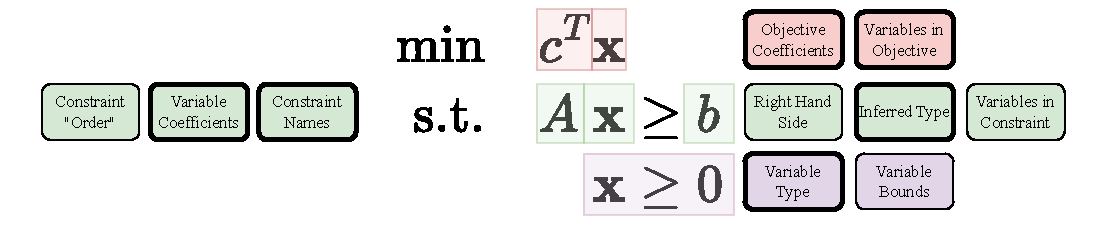
\includegraphics[scale=0.8]{Bilder/DrawIO/model_information}
		\caption{All parts of a model that contain useful information for semantic grouping of constraints and variables. Elements with a thick border are already used as a key concept in one of the existing detectors.}
		\label{fig:tree:information}
	\end{figure}
	
	Before we present 
	
	\clearpage
	
	\section{Motivation}
	% 2 Seiten
	
		A\clearpage
		A\clearpage
	
	\section{Classifiers}
	% 2 Seite
	
		\section{Variable Bounds}
			
			\clearpage
		
		\section{Relaxed MIPLIB types}
		
			\clearpage
			
		\section{Ordered Voting}
		
			\clearpage

	\section{Tree Refinement}
	% 4 Seiten
	
		\begin{figure}[ht!]
			\centering
			\includesvg{Bilder/Hierarchy/hierarchy_binpack_NOP}
			\caption{Test}
			\label{fig:tree:binpackNOP}
		\end{figure}
	
		\clearpage
		A\clearpage
		A\clearpage
		A\clearpage
		
	\section{Strategies}
	
		\subsection{Slice}
			\clearpage
		
		\subsection{Fast}
			\clearpage
		
		\subsection{Recursive}
			\clearpage
		
		\subsection{Finishing}
			\clearpage
	
	\section{Scoring}
	% 1 Seite
	
		\subsection{Entropy Score}
		% 1 Seite
			\clearpage
		
		\subsection{RAND Score}
		% 1 Seite
			\clearpage
		
		\subsection{Connected Block Score}
		% 1 Seite
			\clearpage
